% !TeX encoding = UTF-8
%



\clearpage


	
% Grafikfehler.
	
\subsection*{Anzeigefehler}

Eine kleine Auswahl von Fehlern, die wir durch grafisches Fehlverhalten entdeckten.\\~\\


%\begin{figure}[ht]
%
%	\centering
%	%\label{}
%	
%	\includegraphics[width=\textwidth]{\IssueMedia/}
%	
%	\caption{}
%
%\end{figure}


\begin{figure}[ht]

	\centering
	\label{Anhang:Grafikfehler:Dialog_Pause}
	
	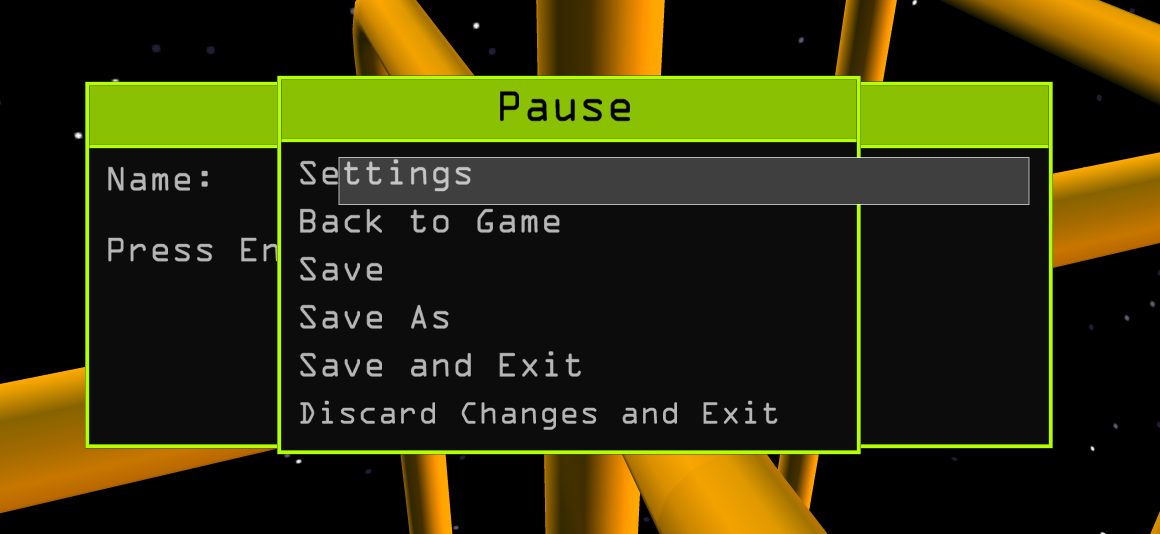
\includegraphics[width=0.9\textwidth]{\IssueMedia/Doppeltes_Menue.png}
	
	\caption{Öffnen eines Pausemenüs während eines Dialogs.}

\end{figure}

\begin{figure}[ht]

	\centering
	\label{Anhang:Grafikfehler:Fenster_Schieben}
	
	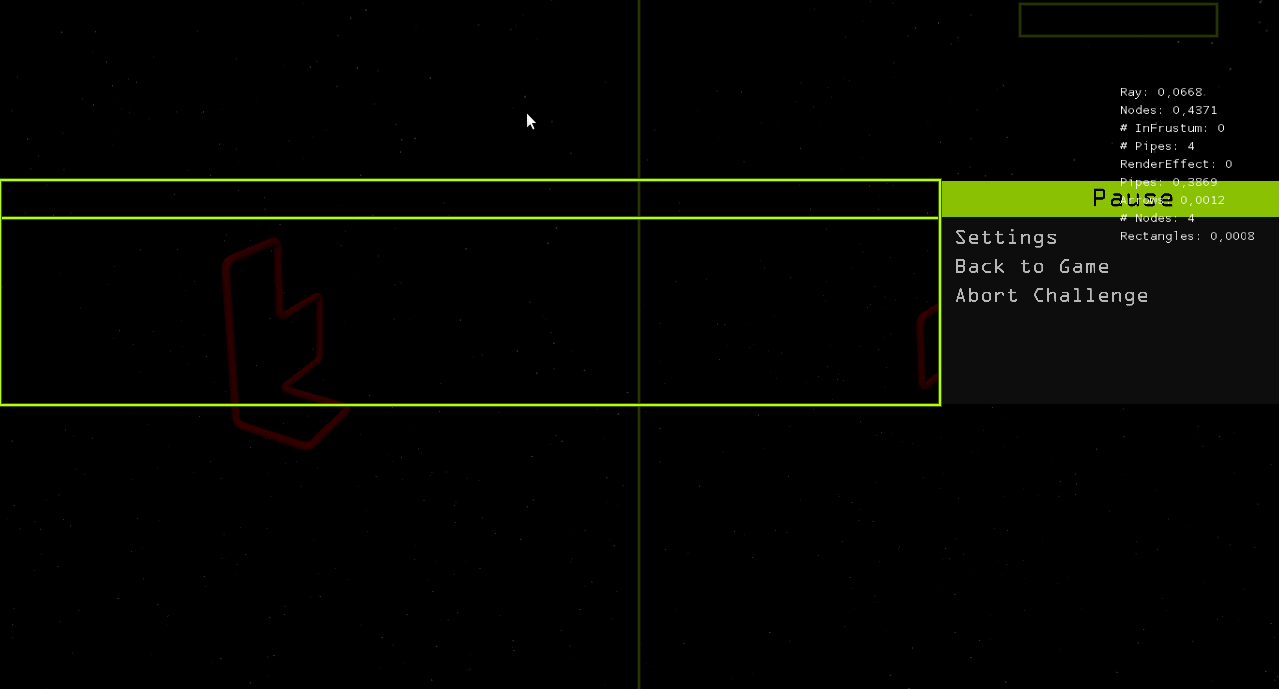
\includegraphics[width=0.9\textwidth]{\IssueMedia/2014-02-04_161034.png}
	
	\caption{Fehlverhalten beim Verschieben eines Fensters.}

\end{figure}



\clearpage



\begin{figure}[ht!]

	\centering
	\label{Anhang:Grafikfehler:Verschmolzene_Geometrie}
	
	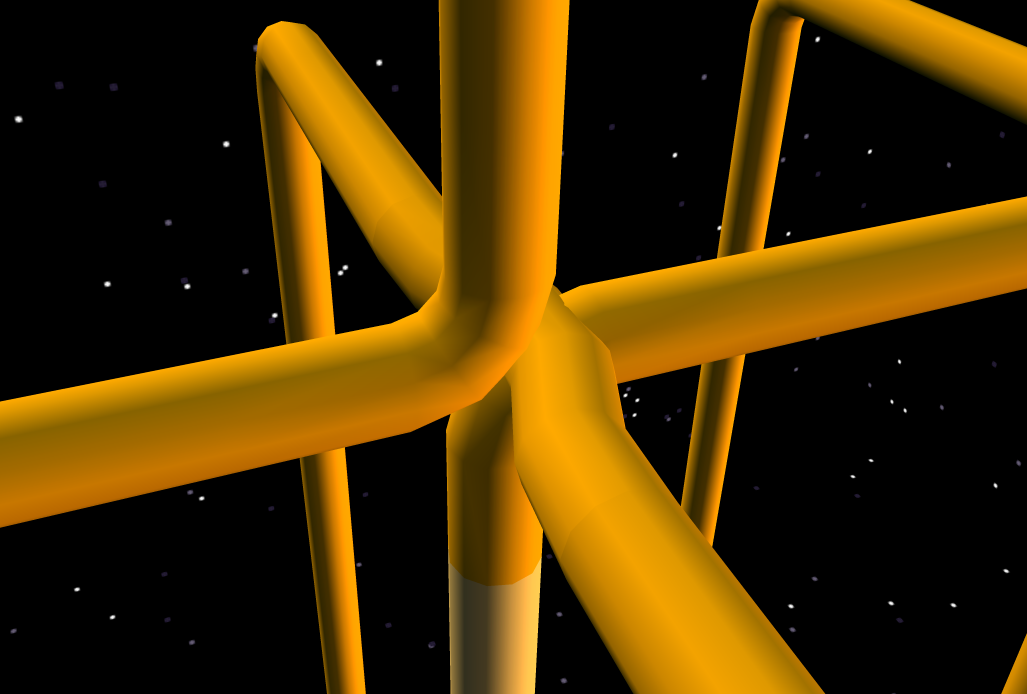
\includegraphics[width=0.9\textwidth]{\IssueMedia/Falscher_Uebergang.png}

\end{figure}


\begin{figure}[ht!]

	\centering
	
	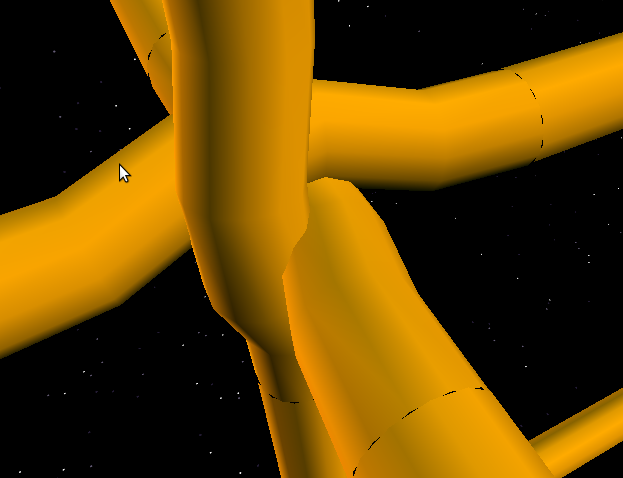
\includegraphics[width=0.9\textwidth]{\IssueMedia/2014-02-03_044044.png}
	
	\caption{Verschmolzene Geometrie an den Übergängen.}

\end{figure}



\clearpage



\begin{figure}[ht]

	\centering
	\label{Anhang:Grafikfehler:Loechrige_Uebergaenge}
	
	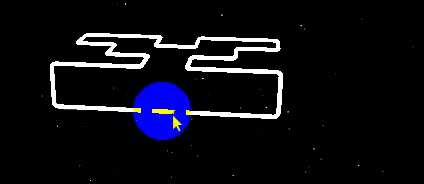
\includegraphics[width=0.9\textwidth]{\IssueMedia/71/8a3fa86f553448f9-75.png}
	
	\caption{Löcher statt Übergänge.}

\end{figure}

